
\begin{figure} [H]
\begin{center}
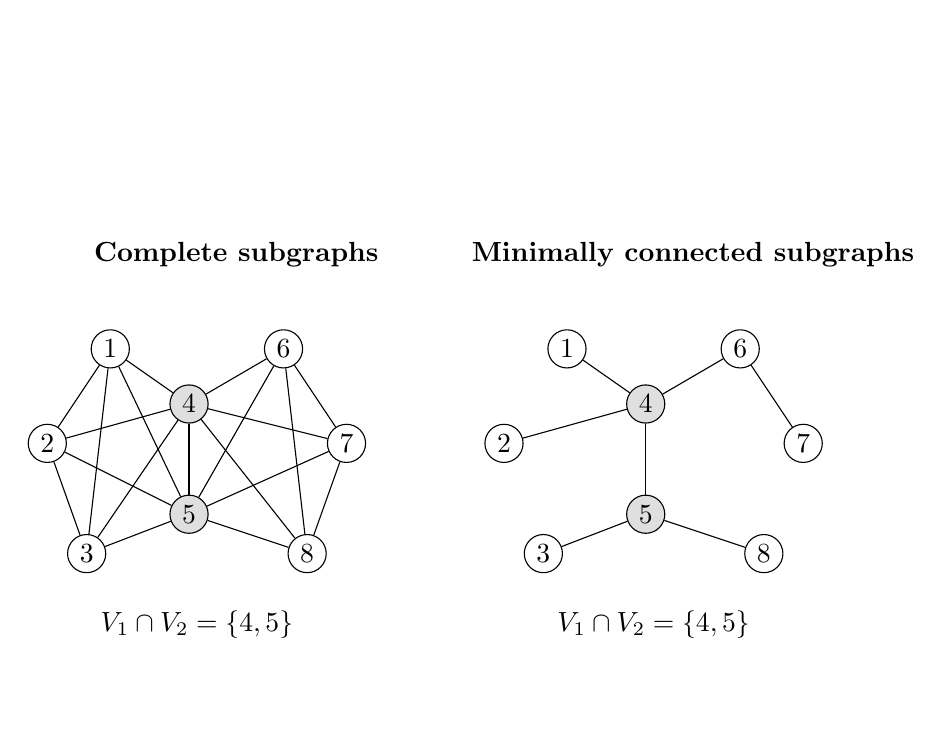
\begin{tikzpicture}[
  scale=1.0,
  every node/.style={circle, draw, fill=white, inner sep=2pt},
  shared/.style={fill=gray!25},
  lab/.style={draw=none, fill=none, font=\bfseries}
]

% =======================
% Panel A: Complete graphs
% =======================
\node[lab] (titleA) at (0,2.6) {Complete subgraphs};

% Nodes (left panel)
\node (A1) at (-1.6, 1.4) {1};
\node (A2) at (-2.4, 0.2) {2};
\node (A3) at (-1.9,-1.2) {3};

\node[shared] (A4) at (-0.6, 0.7) {4};
\node[shared] (A5) at (-0.6,-0.7) {5};

\node (A6) at ( 0.6, 1.4) {6};
\node (A7) at ( 1.4, 0.2) {7};
\node (A8) at ( 0.9,-1.2) {8};

% K5 on {1,2,3,4,5}
\foreach \u/\v in {A1/A2,A1/A3,A1/A4,A1/A5,A2/A3,A2/A4,A2/A5,A3/A4,A3/A5,A4/A5}{
  \draw (\u)--(\v);
}

% K5 on {4,5,6,7,8}
\foreach \u/\v in {A4/A5,A4/A6,A4/A7,A4/A8,A5/A6,A5/A7,A5/A8,A6/A7,A6/A8,A7/A8}{
  \draw (\u)--(\v);
}

\node[lab] at (-0.5,-2.1) {$V_1\cap V_2=\{4,5\}$};

% =======================
% Panel B: Minimal (trees)
% =======================
\node[lab] (titleB) at (5.8,2.6) {Minimally connected subgraphs};

% Nodes (right panel) — same geometry shifted right
\node (B1) at (4.2, 1.4) {1};
\node (B2) at (3.4, 0.2) {2};
\node (B3) at (3.9,-1.2) {3};

\node[shared] (B4) at (5.2, 0.7) {4};
\node[shared] (B5) at (5.2,-0.7) {5};

\node (B6) at (6.4, 1.4) {6};
\node (B7) at (7.2, 0.2) {7};
\node (B8) at (6.7,-1.2) {8};

% Tree on {1,2,3,4,5} (4 edges)
\draw (B4)--(B1);
\draw (B4)--(B2);
\draw (B5)--(B3);
\draw (B4)--(B5);

% Tree on {4,5,6,7,8} (4 edges)
\draw (B4)--(B6);
\draw (B6)--(B7);
\draw (B5)--(B8);
\draw (B4)--(B5);

\node[lab] at (5.3,-2.1) {$V_1\cap V_2=\{4,5\}$};

% =======================
% Caption / statement
% =======================
\end{tikzpicture}
\caption{Same vertex sets $V_1=\{1,2,3,4,5\},V_2=\{4,5,6,7,8\}$ in both panels.
Changing edges (complete vs tree) does not change $V_1\cap V_2$.}
\end{center}

\end{figure}
